% kuleuventheme2 by Janez Kren, September 2017, janez.kren@kuleuven.be, based on:
% kuleuventheme 1.3 by Roland Pastorino, 2013 roland.pastorino@kuleuven.be / www.rolandpastorino.com

\documentclass[11pt,t]{beamer}
\usetheme[sedes]{kuleuven2}	%THEME OPTIONS for LOGO: kul (default), kulak, lrd,    ; OPTIONS for TITLE PAGE: normal (default), sedes


%%% OTHER SETTINGS
\usefonttheme[onlymath]{serif}			% math font with serifs, delete to make it sans-serif
\setbeamertemplate{footline}[body] 		% delete this line to remove footline bar on all frames
%\usepackage[orientation=landscape,size=custom,width=16,height=9,scale=0.5,debug]{beamerposter} %enable for widescreen 16:9 ratio
%\titlegraphic{ \includegraphics[width=.2\paperwidth]{mytitlepagepic.png} } %optional title page image



%%% ADDED PACKAGES:
\usepackage[english]{babel}
\usepackage{amsfonts}
\usepackage{amssymb}
\usepackage{pdfcomment}

% per inserire uno spazio "fantasma" nella definizione di un'abbreviazione
\usepackage{xspace}
%\usepackage{pythontex}

% per inserire un DOI senza problemi coi caratteri "strani" ivi presenti
\usepackage{doi}
\renewcommand{\doitext}{DOI }% originally was "doi:"

% per inserire correttamente le unità di misura SI (incluse quelle binarie)
\usepackage[binary-units]{siunitx}
% se si desidera usare / invece che la potenza -1 per indicare "al secondo"
\sisetup{per-mode=symbol}

% per inserire codice di programmazione complesso
\usepackage{listings}% per inserire codice di programmazione complesso
\lstset{
basicstyle=\ttfamily,
columns=fullflexible,
xleftmargin=3ex,
breaklines,
breakatwhitespace,
escapechar=`
}

% modify some page parameters
\setlength{\parskip}{\medskipamount}

% riga orizzontale
\newcommand{\HRule}{\rule{\linewidth}{0.2mm}}
% esempio di creazione di semplici abbreviazioni
\newcommand{\cas}{\Casper\xspace}

% esempio di creazione di un'abbreviazione con un parametro (il cui uso è indicato da #1)
\newcommand{\cmd}[1]{\texttt{#1}\xspace}
% per citare un RFC, es. \rfc{822}
\newcommand{\rfc}[1]{RFC-#1\xspace}
% per citare un file (es. \file{autoexec.bat}) o una URI fittizia (es. \file{http://www.lioy.it/})
% per le URI vere usare \url o \href
\newcommand{\file}[1]{\texttt{#1}\xspace}
% per inserire codice di esempio in-line
\newcommand{\code}[1]{\lstinline|#1|}
% importante per i pathname Windows perché non si può usare \ essendo un carattere riservato di Latex
\newcommand{\bs}{\textbackslash}
% definizione di un termine: formattazione ed inserimento nell'indice
\newcommand{\tdef}[1]{\textit{#1}\index{#1}}
% meta-termine, usato tipicamente nelle definizioni dei tag
\newcommand{\meta}[1]{\textit{#1}}

\newcommand{\pdfnote}[1]{\marginnote{\pdfcomment[icon=note]{#1}}}


%%PERSONAL CMD
\newcommand{\bt}[1]{\textbf{#1}}  %%bold text
\newcommand{\ita}[1]{\textit{#1}}  %%italic text
\newcommand{\bit}[1]{\textbf{\textit{#1}}}
\newcommand{\ie}{i.e.\xspace}
\newcommand{\eg}{e.g.\xspace}
\newcommand{\sed}{  %insert logo sedes on the bottom right of page
	\begin{tikzpicture}[remember picture,overlay]
		\node [anchor=south east,inner sep=0pt, yshift=.05\paperheight, , opacity=0.5] at (current page.south east) 
		{
\includegraphics[height=.3\paperheight]{graphics/sedes.png} };
	\end{tikzpicture}
}

%\newcommand{\pic}[2]{
%\begin{pycode}
 % import os
  %directory = "root/images"
  %extension = ".png"
  %#files = [file for file in os.listdir(directory) if 
 %# file.lower().endswith(extension)]
  %#for file in files:
  
   %  print(r"\begin{figure}[h]")
    % print(r"\centering")
     %print(r"\includegraphics[width=0.5]\linewidth]{%s}" %file)
     %print(r"\caption[%s]{ %s}" %file)
     %print(r"\label{fig:{%s}" %file)
     %print(r"\end{figure:{%s}"%file)
  %\end{pycode}
%}


\usepackage{hyperref}
\UseRawInputEncoding  %to use UTF-8 Encoding
\hypersetup{%
    pdfpagemode={UseOutlines},
    bookmarksopen,
    pdfstartview={FitH},
    colorlinks,
    linkcolor={black},
    citecolor={red},
    urlcolor={blue}
  }


%%% TITLE PAGE INFO:
\title[Security Analysis of the WPA2 KRACK patches]{Security Analysis of the WPA2 KRACK patches} %[]] will appear in footline
\subtitle{Study Case}

\author{\bt{Graziano Marallo}}
\institute{KU Leuven}
\date{13 December 2018}
	


\begin{document}
\csname beamer@calculateheadfoot\endcsname %recalculate head and foot dimension

 %%
 %%  0. TITLE PAGE and TABLE OF CONTENT
 %%
\begin{frame}[plain,noframenumbering]
	\titlepage
\sed
\end{frame}
	

% Table of Contents
\begin{frame}{Outline}
	\hfill	{\large \parbox{.961\textwidth}{\tableofcontents[hideothersubsections]}}
		\marginnote{\pdfcomment[icon=note]{Greetings to the audience}}
\sed
\end{frame}


\begin{frame}[fragile]{Introduction} 
	

		\begin{itemize}
			\item Most of the Wi-Fi networks which are used today are protected and secured by the WPA2
			\item Used everywhere
			\item Can we trust WPA2?
			\item Is really secure as we thought?
		\end{itemize}
	
		\pdfnote{	- WPA2: Wi-Fi Protected Access 2 \\
	So every router, smartphone, laptop and smart device
	that is on the market, is using this kind of protocol to get connect to the internet and exchange data. Nowadays those data are becoming more crucial and 
	important than in the past 
	All the aspects of our lives are driven and covered by those data that are exchanged on the network.
	Now what if we discover that all our data are not exchanged in secure manner anymore?
	What if a protocol thought be secure for over 14 years turned out be not secure anymore?
	Are there any change to understand and possibly mitigate the problem? In order to address these question 
	a proper analysis has to be done.}

\sed
\end{frame}


%%%%%%%%%%%%%%%%%%%%%%%% END OF OUTLINE %%%%%%%%%%%%%%%%%%%%%%%%%%%

 %%
 %%  SECTION 1 - 4-WAY HANDSHAKE
 %%
 \section{4-Way Handshake Protocol } 
 \begin{frame}[fragile]{4-Way Handshake Protocol \tiny\cite{asc}}  
	
	\begin{itemize}
		\item Provides mutual authentication between client and server
		\item Negotiates a fresh PTK, proven to be secret
		\item The protocol itself proven to be secure
	\end{itemize}
	
	\pdfnote{Say why 4hw is important and its basica charateristcs}
 \sed
 \end{frame}

 \begin{frame}[fragile]{Functioning}  
	
	\begin{itemize}
		\item It is composed of 5 different stages:
		\begin{itemize}
			\item Stage 1: \textit{Network Discovery}
			\item Stage 2: \textit{Authentication and Association}
			\item Stage 3: \textit{802.1x Authentication} 
			\item Stage 4: \textit{4-Way Handshake}  
			\item Stage 5: \textit{Group Key Handshake} 
		\end{itemize}
		\item Stage 4 is composed of 4 messages exchanged between supplicant and authenticator
		\item During this exchange the actual protocol is performed
	\end{itemize}


 \sed
 \end{frame}

 \begin{frame}[fragile]{Message exchange: Msg 1}  
	%%%%%%TODO: NOTES 
	\marginnote{\pdfcomment[icon=note]{
		Message integrity check \\ 
		Nonce = number randomly generate only once
	}}
	\begin{figure}[tbh]
		\centering
		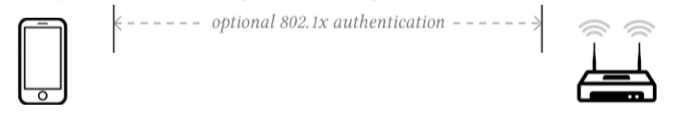
\includegraphics[width=0.8\linewidth]{graphics/4wh/phase1.png}
		\label{fig:phase1}
	  \end{figure}
	
	\begin{itemize}
		\item Sent by the authenticator 
		\item Contains a randomly generated ANonce 
		\item No protection by MIC
		\item Possible message forging
	\end{itemize}


 \end{frame}

 \begin{frame}[fragile]{Message exchange: Msg 2}  
	
	\begin{figure}[tbh]
		\centering
		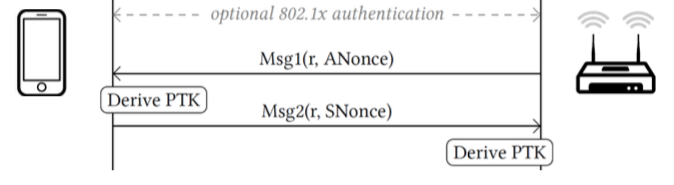
\includegraphics[width=0.8\linewidth]{graphics/4wh/phase2.png}
		\label{fig:phase2}
	  \end{figure}
	  \begin{itemize}
		\item Sent by the supplicant 
		\item Contains the random SNonce of supplicant
		\item Protection by MIC
		\item Computes PTK
	\end{itemize}

	\pdfnote{Pairwise temporary key to ensure authentication and authorisation}

 \sed
 \end{frame}

 \begin{frame}[fragile]{Message exchange: Msg 3}  
	
	\begin{figure}[tbh]
		\centering
		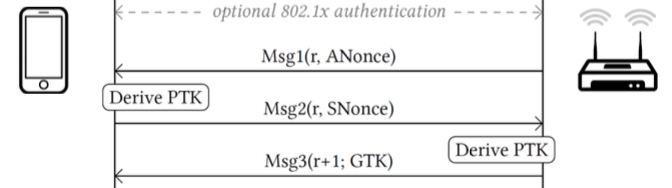
\includegraphics[width=0.8\linewidth]{graphics/4wh/phase3.png}
		\label{fig:phase3}
	  \end{figure}

	  \begin{itemize}
		\item Sent from the authenticator in response to the supplicant
		\item Contains again ANonce 
		\item RSNE is checked with the one received when the protocol \\takes place for the first time
	\end{itemize}

	\pdfnote{it's important to say that in the Key Data Field of the EAPOL message is stored
	the RSNE element, that contains the cipher suite chosen by the supplicant in the association request sent before. Once the authenticator has received this message, is able to calculate the PTK, verify the MIC and check if any miss-match occurs 
	between the old RSNE and the fresh one that has been received. If any discrepancy occurs, the protocol is aborted instantly.}
 \sed
 \end{frame}

 
 \begin{frame}[fragile]{Message exchange: Msg 4}  
	
	\begin{figure}[tbh]
		\centering
		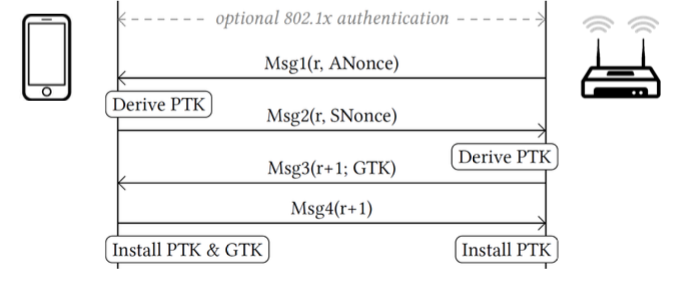
\includegraphics[width=0.8\linewidth]{graphics/4wh/phase4.png}
		\label{fig:phase4}
	  \end{figure}

	  \begin{itemize}
		\item Last message sent by the supplicant in order to inform the authenticator that the handshake has been completed
		\item Protection by MIC
		\item Encrypted data frame can be transmitted
	\end{itemize}

 \sed
 \end{frame}

%%%%%%%%%%%%%%%%%%%%%%%% END OF SECTION 1 %%%%%%%%%%%%%%%%%%%%%%%%%%%

%%
 %%  SECTION 2 - KRACK
 %%
\section{KRACK}
\begin{frame}[fragile]{KRACK \tiny\cite{krk}}  
	
	\begin{figure}[tbh]
		\centering
		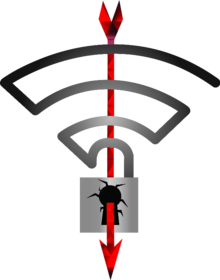
\includegraphics[width=0.3\linewidth]{graphics/krack/kracklogo.png}
		\label{fig:kracklogo}
	  \end{figure}

	\begin{itemize}
		\item The supplicant still accepts retransmissions of message 3
		\item Possibility to force the reinstallation of th PTK 
	\end{itemize}
	\pdfnote{ Krack abuses of a protocol to reinstall an already in-use key 
	by resetting the nonces and/or the replay counters associated to it.\\
	the adversary can trick a victim in reinstalling an already in-use key without be conscious of it}

\sed
\end{frame}

\begin{frame}[fragile]{Scenario}  
	If we consider the victim still accepting retransmission of message 3 after the session 
	key has been installed, the attack is pretty straightforward

	\begin{figure}[tbh]
		\centering
		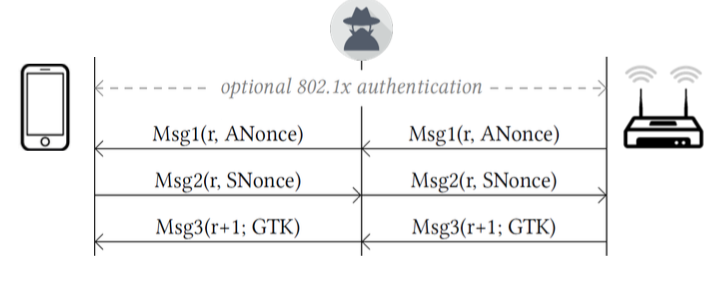
\includegraphics[width=0.6\linewidth]{graphics/krack/k1.png}
		\label{fig:k1}
	  \end{figure}

	In the first stage:
	\begin{itemize}
	\item The attacker manage to set up a channel-based MitM attack
	\item Able to sniff traffic and manipulate it
	\end{itemize}

\sed
\end{frame}

\begin{frame}[fragile]{Scenario}  

	\begin{figure}[tbh]
		\centering
		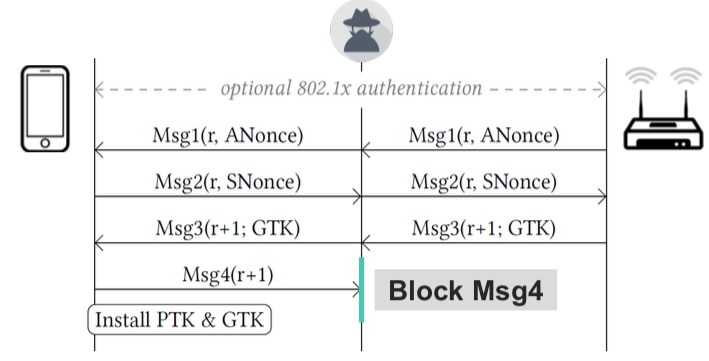
\includegraphics[width=0.7\linewidth]{graphics/krack/k2.png}
		\label{fig:k2}
	  \end{figure}

	In the second stage:
	\begin{itemize}
	\item The attacker can prevent message 4 from arriving to the authenticator
	\item The supplicant will install PTK and GTK as soon as \\message 4 is sent
	\end{itemize}

\sed
\end{frame}

\begin{frame}[fragile]{Scenario}  

	\begin{figure}[tbh]
		\centering
		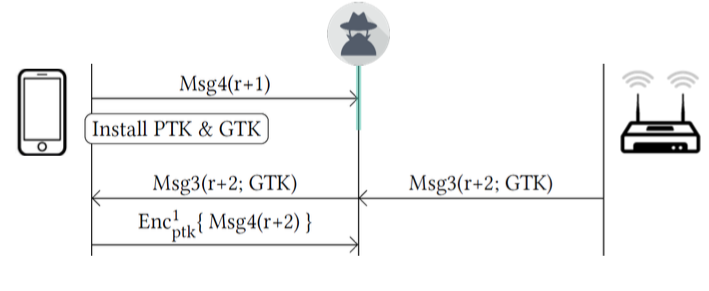
\includegraphics[width=0.9\linewidth]{graphics/krack/k3.png}
		\label{fig:k3}
	  \end{figure}

	In the third stage:
	\begin{itemize}
	\item Authenticator will resend message 3 
	\item Victim is inducted to reinstall 
	\item Both replay counter and nonce are reset
	\end{itemize}

\sed
\end{frame}

\begin{frame}[fragile]{Scenario}  
	\begin{columns}[t]
		\begin{column}{.5\textwidth}
			In the fourth stage:
			\begin{itemize}
				\item Supplicant will send an encrypted message since the key has been reinstalled
				\item Authenticator will accept an old unencrypted message 4 which has a replay counter r + 1
				\item PTK will be installed and the AP will start sending encrypted unicast data frames to the client
			\end{itemize}
		\end{column}


		\begin{column}{.5\textwidth}
			\begin{figure}[tbh]
				\centering
				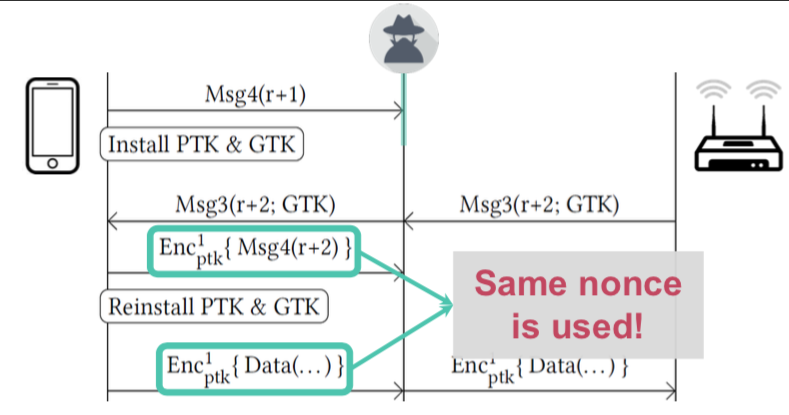
\includegraphics[width=1.0\linewidth]{graphics/krack/k4.png}
				\label{fig:k4}
			\end{figure}
		\end{column}
	
	\end{columns}	

	\pdfnote{In principle this should happen but carefully analyzing the 802.11 standard has been noticed that the authenticator may actually
	accept \textit{any} replay counter used in the 4wh previously. Basically some APs accept replay counters that were used in a message to the client, but were not yet used in a reply from the client. In that way those APs will accept
	the older unencrypted message 4 which has a replay counter r + 1, as showed in figure}

\sed
\end{frame}

\begin{frame}[fragile]{Scenario}  
	\begin{columns}[t]
		\begin{column}{.5\textwidth}
			\begin{figure}[tbh]
				\centering
				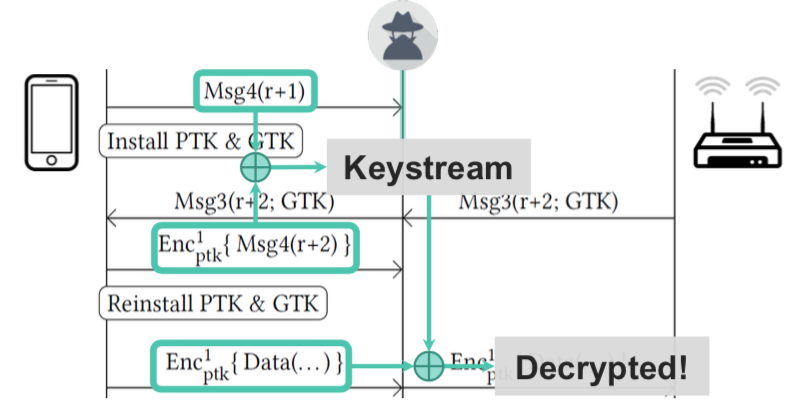
\includegraphics[width=1.1\linewidth]{graphics/krack/k5.png}
				\label{fig:k4}
			  \end{figure}
		
		\end{column}
	
		\begin{column}{.5\textwidth}
			In the end:
			\begin{itemize}
			\item When the victim retransmit its next data frame, the data-confidentiality protocol will reuse nonces
			\item The attacker can manages both the forwarding time between messages and amount of nonces
			\item The client could be de-authenticated by the attacker himself
			\end{itemize}
		\end{column}
	\end{columns}	


\sed
\end{frame}

%%%%%%%%%%%%%%%%%%%%%%%% END OF SECTION 2 %%%%%%%%%%%%%%%%%%%%%%%%%%%

 %%
 %%  SECTION 3 - FUZZING 
 %%
\section{Fuzzing}

\begin{frame}[fragile]{Fuzzing \tiny\cite{fzn}}  
Various technique can be used to fight hackers' attacks like static analysis, dynamic, symbolic execution and fuzzing.
Focus our attention on the latter:
	\begin{itemize}
		\item Fuzzing requires less knowledge of the target, 
		\item Easily adapted and scaled to a large variety of situation and problem. 
		\item The most popular vulnerability discovery solution nowadays
	\end{itemize}
\sed
\end{frame}

\begin{frame}[fragile]{Fuzzing process}  

	\begin{figure}[tbh]
		\centering
		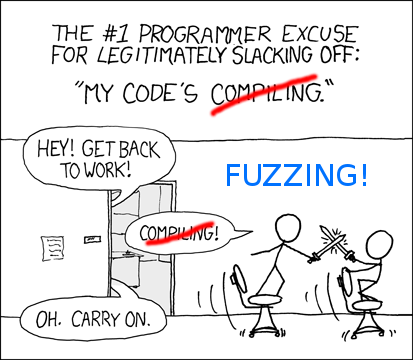
\includegraphics[width=0.3\linewidth]{graphics/fuzzing/fuz.png}
		\label{fig:fuz}
		\caption{Fuzzing \tiny\cite{img}}
	  \end{figure}

	\begin{itemize}
		\item Starts with generating massive normal and abnormal inputs towards application
		\item Try to detect exception by feeding generated inputs \\to the target applications
		\item Monitor each execution states
	\end{itemize}
\sed
\end{frame}


\begin{frame}[fragile]{Fuzzing} 
The main process of the traditional fuzzing process has 4 main stages
\begin{columns}[t]
	\begin{column}{.5\textwidth}
		\begin{itemize}
			\item Test case generation stage
			\item Test case running stage
			\item Program execution stage monitoring
			\item Analysis of exceptions
			\end{itemize}	
	\end{column}

	\begin{column}{.5\textwidth}
		\begin{figure}[tbh]
			\centering
			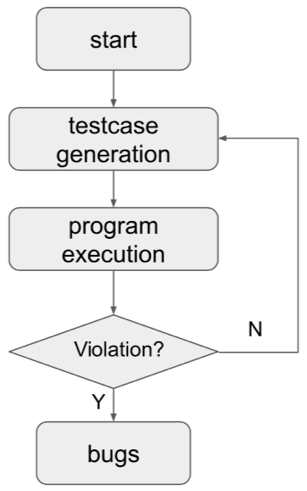
\includegraphics[width=0.6\linewidth]{graphics/fuzzing/fuzz_stages.png}
			\label{fig:fuzz_stages}
		  \end{figure}
	\end{column}
\end{columns}	

\sed
\end{frame}


\begin{frame}[fragile]{American Fuzzy Lop}  
	
	\begin{itemize}
		\item \textbf{Brute-force Fuzzer} 
		\item Coupled with an exceedingly simple but rock-solid instrumentation-guided genetic algorithm
		\item Uses a modified form of edge coverage 
	\end{itemize} 
	 
	\pdfnote{it works by instrumenting the code and marking each that could be useful to anlyse. In this way what we got 
	is basically a good coverage of the code under anlysis that allows to find significant results.}
\sed
\end{frame}

\begin{frame}[fragile]{Algorithm} 
How it works:
\begin{enumerate}
  \item Load user-supplied initial test cases into the queue,
  \item Take next input file from the queue,
  \item Attempt to trim the test case to the smallest size that doesn't alter the measured behaviour of the program,
  \item Repeatedly mutate the file using a balanced and well-researched variety of traditional fuzzing strategies,
  \item If any of the generated mutations resulted in a new state transition recorded by the instrumentation, add mutated output as a new entry in the queue.
  \item Go to 2.
\end{enumerate}

\pdfnote{}

\sed
\end{frame}



%%%%%%%%%%%%%%%%%%%%%%%% END OF SECTION 3 %%%%%%%%%%%%%%%%%%%%%%%%%%%


 %%
 %%  SECTION 4 - GOAL 
 %%
 \section{Goal \& Findings} 
 \begin{frame}[fragile]{Goal}  
	Goal of the research:
	\begin{itemize}
		\item Identify the source of the problem
		\item Perform several analysis
		\item Debug the source code 
		\item Analyse with a systematic approach the protocol
		\item Try to solve or mitigate the problem
		\item Propose a possible solution
	\end{itemize}

 \sed
 \end{frame}

  
 \begin{frame}[fragile]{Ideas}  
	\begin{itemize}
		\item Analyse source code of IWD (open source implementation of the 4WH)
		\item Find a possible spot where to inject dummy input
		\item Create an harness code
		\item Start fuzzing 
	\end{itemize}
 \sed
 \pdfcomment{iNet Wireless Daemon (aka iwd) project aims to provide a comprehensive Wi-Fi connectivity solution for Linux based devices, and
 it has been written by Intel basically with aim of replacing WPA Supplicant.}
 \end{frame}


 \begin{frame}[fragile]{Findings}  

	\begin{itemize}
		\item  TODO 
	\end{itemize}

 \sed
 \end{frame}

%%%%%%%%%%%%%%%%%%%%%%%% END OF SECTION 4 %%%%%%%%%%%%%%%%%%%%%%%%%%%

%%%%%%%%%%%%%%%%%%%%%%%% BIBLIOGRAPY & THANKS %%%%%%%%%%%%%%%%%%%%%%%%%%%

\begin{frame}[c,plain,noframenumbering]
\begin{tikzpicture}[remember picture,overlay]
\fill[fill=kul-blue]
    (current page.south east)  rectangle  ([shift={(0,-0.1\paperheight)}]current page.north west)   ;
\end{tikzpicture}

\centering
\LARGE\textcolor{white}{\bt{Thanks for the attention!}}
\end{frame}



\appendix
\begin{frame}[noframenumbering,label=extraframe]{Bibliography}
% !TEX encoding = IsoLatin

% La bibliografia, da inserirsi solo se ci sono state citazioni.
% In questo caso ricordarsi che bisogna sempre elaborare due volte il file .TEX
% perch� la prima volta viene generata la bibliografia mentre la seconda volta viene inclusa

% NOTA: citare il DOI non � obbligatorio ma MOLTO desiderabile

\begin{thebibliography}{9} % se ci sono meno di 10 citazioni
%\begin{thebibliography}{99} % se ci sono da 10 a 99 citazioni
%\begin{thebibliography}{999} % se ci sono da 100 a 999 citazioni

%%ASIACS PAPER
%citation on paper
\bibitem{asc}
%author
Vanhoef, M and Schepers, D and Piessens, F,
%title
``Discovering logical vulnerabilities in the Wi-Fi handshake using model-based testing'',
% name of the journa�
ASIA CCS 2017 - Proceedings of the 2017 ACM Asia Conference on Computer and Communications Security,
% %volume and number of the journal (may not be present)
%Vol.\ 1,
% year and month of publishing
2017,
% page of the article
pp.\ 360-371,
% DOI
\doi{110.1145/3052973}


\bibitem{krk}
% nome del progetto
OPCDE, Dubai, 7 April 2018, Vanhoef
 % URI della pagina web
\url{https://papers.mathyvanhoef.com/opcde2018-slides.pdf}



%%FUZZING PAPER
\bibitem{fzn}
Li, Jun and Zhao, Bodong and Zhang, Chao,
``Fuzzing: a survey'',
Cybersecurity,
Vol.\ 1,
2018,
pp.\ 1-13,
\doi{10.1186/s42400-018-0002-y}


\bibitem{img}
% nome del progetto
Fuzzing image
 % URI della pagina web
\url{https://medium.com/@dieswaytoofast/fuzzing-and-deep-learning-5aae84c20303}



\end{thebibliography}



\end{frame}


\end{document}